\section{Validação computacional exata}
\label{sec:numerical}

\subsection{Implementação}

O script
\path{reproducibility/selecao/seletor_dinamico_exato.py}
implementa os \cref{alg:fixed-tree,alg:variable-tree}. O domínio numérico é
\texttt{Fraction}. As tabelas são dicionários esparsos indexados
por pares de \texttt{Fraction}; a junção dos filhos usa igualdade racional
exata no valor $w$. Perdas, penalidades, comparações de objetivo, alturas,
endereços $\Gamma^\sharp$ e desempates não usam ponto flutuante.
\texttt{NumPy} e \texttt{Matplotlib} aparecem somente depois da seleção, para
desenhar as figuras.

Cada execução verifica:
\begin{enumerate}[label=(\alph*),leftmargin=2em]
 \item a continuidade de todas as fronteiras da montagem vencedora;
 \item a altura de cada folha;
 \item a igualdade entre o ótimo da recorrência variável e o mínimo obtido ao
 enumerar separadamente todas as formas e resolver cada árvore fixa;
 \item a coincidência com uma enumeração direta de representações na
 instância mínima descrita abaixo;
 \item que uma derivação separada de $\mathcal Q_H$, dos pares de extremos
 e das perdas locais coincide com as rotinas usadas pela PD;
 \item as recorrências com número exato de folhas e de gargalo contra
 enumeração sem poda;
 \item a robustez da comparação num orçamento sem células eliminadas;
 \item que o valor exato não excede os valores das três referências.
\end{enumerate}

O verificador de (d) é independente da \emph{recorrência}, mas reutiliza o
catálogo local e a função de perda. Por isso (e) constitui uma segunda camada:
ela enumera $\mathcal Q_H$ diretamente pelas frações reduzidas, forma os pares
de extremos a partir de $(y_0,s)$ sem chamar o dicionário da PD e recompõe
\eqref{eq:local-loss} pela fórmula afim nos pontos observados. As duas
comparações possuem, assim, implementações independentes do dicionário e da
perda. O teste de erro uniforme em (f) usa $f\equiv0$, caso em que
$e_f(J;u,v)=\max\{|u|,|v|\}$ é calculado exatamente.

\subsection{Auditoria por enumeração direta}

Na instância de auditoria, tomam-se $(D,H)=(1,2)$, as cinco observações
racionais $x_i\in\{0,\tfrac14,\tfrac12,\tfrac34,1\}$ do alvo $2|x-1/2|$ e as
penalidades $\lambda_{\rm bits}=\tfrac1{200}$,
$\lambda_{\rm split}=\tfrac1{50}$. Há $42$ átomos admissíveis na
raiz. O verificador examina diretamente os $42$ candidatos de uma folha e
todos os $42^2=1764$ pares de átomos dos filhos, descartando os $1704$ pares
que não coincidem em $x=1/2$. Restam $60$ subdivisões contínuas, ou $102$
representações ao contar também as folhas. O custo e o fluxo vencedores
coincidem bit a bit com a programação dinâmica.

Nessa instância, como na instância principal, o minimizador de custo é único,
de modo que ela não chega a exercitar o desempate \eqref{eq:tie-key}. O script
inclui por isso três cenários dedicados, nos quais o vencedor da recorrência é
confrontado com a minimização exaustiva da chave completa sobre todas as
representações contínuas, enumeradas \emph{sem} poda por estado:
\begin{enumerate}[label=(\alph*),leftmargin=2em]
 \item com dados e penalidades nulos e $(D,H)=(1,2)$, todas as $102$
 representações têm custo zero e a seleção é decidida pelo comprimento do
 fluxo;
 \item o mesmo com $(D,H)=(2,3)$, em que as $1370$ representações contínuas
 empatam em custo, o que exercita dois níveis de concatenação;
 \item com dados identicamente nulos e $(D,H)=(2,3)$, dois candidatos empatam
 simultaneamente em custo e em comprimento, e a seleção é decidida pela ordem
 lexicográfica do fluxo.
\end{enumerate}
Nos três casos a recorrência devolve exatamente o mesmo fluxo que a
minimização exaustiva, o que verifica a compatibilidade de \eqref{eq:tie-key}
com a concatenação afirmada no \cref{thm:fixed-correctness}.

Para testar a \cref{sec:hard-budgets}, o script enumera sem poda todas as
$1370$ representações contínuas de $(D,H)=(2,3)$. Para cada número viável de
folhas e cada par de estados externos, compara tanto o melhor custo aditivo
$C_{d,n}$ quanto o melhor gargalo $B_{d,n}$ com a enumeração completa. Também
compara, para cada $N\in\{1,2,3,4\}$, o ótimo com no máximo $N$ folhas. Todas
as igualdades são verificadas em aritmética racional exata.

\begin{table}[t]
 \centering
 \caption{Verificações executáveis das duas instâncias.}
 \label{tab:dp-audit}
 \small
 \begin{tabularx}{\linewidth}{@{}Xr@{}}
\toprule
Verificação & resultado \\
\midrule
Dicionário/perdas derivados das definições & true \\
Enumeração direta $(D,H)=(1,2)$ & true \\
Pares de subárvores examinados diretamente & 1764 \\
Formas de árvore enumeradas na instância principal & 26 \\
Formas de árvore com catálogo não vazio & 11 \\
Células da árvore completa sem átomo admissível & 4 \\
DP variável $=$ mínimo sobre formas fixas & true \\
Empates de custo máximos resolvidos pela chave & 1370 \\
DP $=$ mínimo exaustivo sob empate & true \\
Fórmula geométrica (1350 casos) & true \\
Orçamento de folhas $=$ enumeração exaustiva & true \\
Gargalo uniforme $=$ enumeração exaustiva & true \\
Ótimo exato não pior que as três referências & true \\
\bottomrule
\end{tabularx}

\end{table}

As contagens e os fluxos da \cref{tab:dp-audit} coincidem com a enumeração
exaustiva independente em todas as instâncias indicadas, inclusive para a
recorrência de gargalo do \cref{thm:bottleneck}.

\subsection{Instância de regressão e rotas de controle}

O experimento a seguir é uma regressão interna de correção, não um estudo de
desempenho nem uma comparação empírica de métodos. As três rotas auxiliares
servem somente como candidatos admissíveis cujo custo exato deve ser maior ou
igual ao ótimo da programação dinâmica. Não se inferem velocidade, qualidade
estatística ou superioridade prática a partir desta única instância sintética.

A instância principal usa $K=[0,1]$, $(D,H)=(3,4)$ e as $17$ observações
diádicas $x_i=i/16$ do alvo racional
\begin{equation}
 f(x)=\frac{1}{1+16(x-\tfrac14)^2}.
 \label{eq:experiment-target}
\end{equation}
As penalidades são
\[
 \lambda_{\rm bits}=\frac1{500},
 \qquad
 \lambda_{\rm split}=\frac1{100}.
\]
Há $23$ valores racionais e $22$ inclinações não nulas de altura no máximo
$4$, isto é, $506$ átomos por célula geometricamente admissível. A árvore
completa possui $15$ células, das quais $11$ são admissíveis: pela
\cref{prop:translation-obstruction}, as quatro células de profundidade $3$ que
cobrem $[\tfrac12,1]$ têm $m\in\{4,5,6,7\}$ e nenhum átomo de altura no
máximo $4$. Consequentemente, das $26$ formas de árvore de profundidade no
máximo $3$, apenas $11$ admitem alguma rotulação contínua; as $15$ restantes
--- todas as que subdividem a metade direita até a profundidade $3$ --- têm
catálogo vazio. As $26$ formas são enumeradas para auditoria, e o mínimo sobre
as viáveis coincide com a recorrência variável. A tabela esparsa da raiz
contém $3383$ estados realizáveis.

Essa assimetria deve ser mantida em vista ao ler a tabela: nesta instância a
metade esquerda do domínio é refinável até a profundidade $3$ e a metade
direita apenas até a profundidade $2$.

As rotas de controle são definidas sob o mesmo funcional:
\begin{itemize}[leftmargin=1.7em]
 \item \emph{malha uniforme}: escolhe o melhor entre as árvores completas de
 profundidades $0,1,2,3$, rotulando cada uma exatamente. Nesta instância a
 profundidade $3$ é \emph{inviável} --- sua metade direita não admite
 rotulação alguma ---, de modo que a escolha se dá de fato entre as
 profundidades $0$, $1$ e $2$, com objetivos $0{,}565803$, $0{,}572135$ e
 $0{,}376159$; vence a profundidade $2$, com quatro folhas;
 \item \emph{adaptativo certificado}: subdivide quando
 $M(J)|J|^2/8>\varepsilon_I$ e depois rotula a árvore exatamente; para
 \eqref{eq:experiment-target},
 \[
 f''(x)=
 \frac{32\bigl(48(x-\tfrac14)^2-1\bigr)}
      {\bigl(1+16(x-\tfrac14)^2\bigr)^3},
 \]
 e o máximo local é calculado racionalmente nos pontos críticos. O programa
 percorre $\varepsilon_I\in\{2^{-1},\dots,2^{-10}\}$ e retém o melhor
 resultado sob o mesmo objetivo da regressão; o caso retido é
 $\varepsilon_I=\tfrac12$. Registre-se que esse ajuste favorece a referência,
 e que apertar o certificado não ajuda: $\varepsilon_I\in\{2^{-3},2^{-4}\}$
 produz seis folhas e objetivo $0{,}571837$, e $\varepsilon_I\le2^{-5}$ exige
 uma árvore fora do catálogo;
 \item \emph{guloso}: começa na raiz, testa cada subdivisão de uma única folha,
 reotimiza exatamente todos os rótulos da árvore candidata e aceita apenas
 uma redução imediata do objetivo.
\end{itemize}

\begin{table}[t]
 \centering
 \caption{Regressão sob o mesmo custo racional. Os decimais arredondam a seis
 casas as frações brutas dos campos \texttt{loss\_exact} e
 \texttt{cost\_exact} do arquivo suplementar \texttt{resultados.json}.
 ``Erro quadrático'' é a soma ponderada dos resíduos quadráticos, não a sua
 média; a tabela não constitui um benchmark de desempenho.}
 \label{tab:selector-comparison}
 \small
 \begin{tabular}{lrrrr}
\toprule
Método & folhas & erro quadrático & bits & objetivo \\
\midrule
Ótimo exato & 3 & 0.041497 & 84 & 0.229497 \\
Malha uniforme & 4 & 0.116159 & 115 & 0.376159 \\
Adaptativo certificado & 3 & 0.041497 & 84 & 0.229497 \\
Heurística gulosa & 1 & 0.517803 & 24 & 0.565803 \\
\bottomrule
\end{tabular}

\end{table}

As frações brutas mencionadas na legenda estão no arquivo
\texttt{resultados.json}, no diretório \texttt{reproducibility/selecao}.

O ótimo exato possui três folhas:
\[
 [0,\tfrac14],\qquad[\tfrac14,\tfrac12],\qquad[\tfrac12,1],
\]
com valores nodais
\[
 \frac12,\quad1,\quad\frac12,\quad0.
\]
Suas inclinações são $2,-2,-1$ e sua altura máxima é $4$. O refinamento
certificado com $\varepsilon_I=\tfrac12$ coincide com essa árvore nesta
instância. A coincidência é registrada como propriedade deste caso de teste.
A melhor malha uniforme viável usa quatro folhas e tem
custo maior. A heurística gulosa permanece na raiz: a única subdivisão isolada
disponível eleva o objetivo de $0{,}565803$ para $0{,}572135$, embora duas
subdivisões coordenadas o reduzam para $0{,}229497$. O exemplo torna
visível a razão algorítmica para preservar estados e subproblemas em vez de
tomar apenas decisões locais.

\begin{figure}[t]
 \centering
 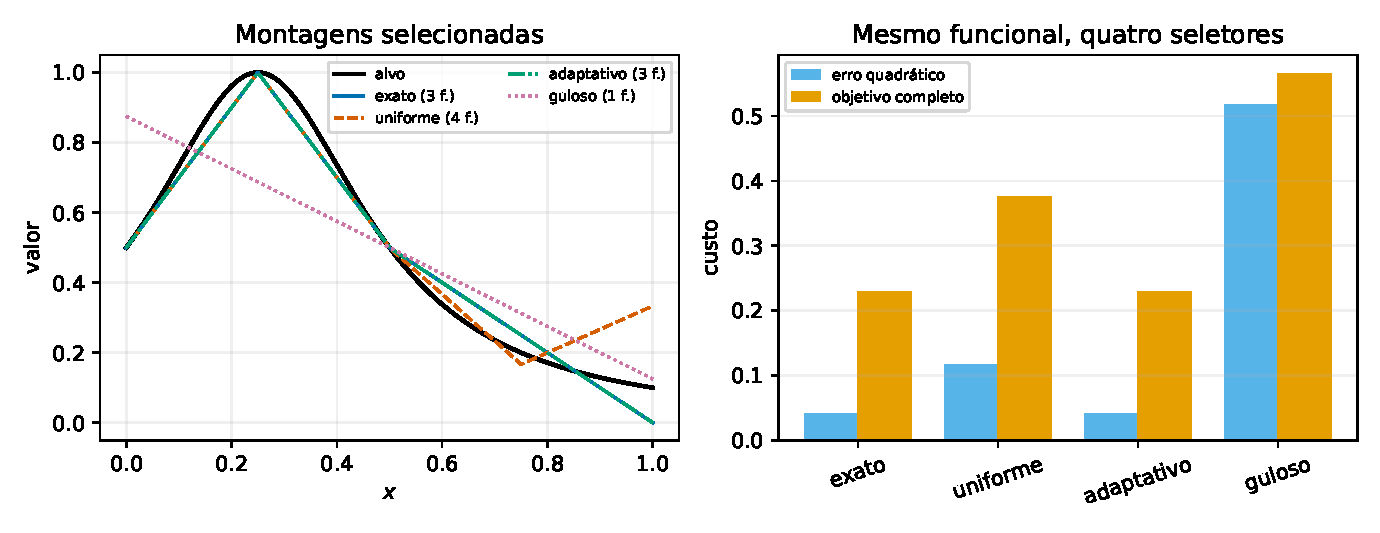
\includegraphics[width=\linewidth]{fig02_comparacao_seletores.pdf}
 \caption{À esquerda, o alvo e as quatro montagens. À direita, erro
 quadrático e objetivo completo. Todas as decisões foram tomadas com
 racionais exatos; o ponto flutuante é usado somente no desenho. A figura é
 um diagnóstico de regressão, não uma comparação de eficiência.}
 \label{fig:selector-comparison}
\end{figure}

O resultado visual da regressão aparece na
\cref{fig:selector-comparison}; os valores exatos correspondentes estão na
\cref{tab:selector-comparison}.

\subsection{Propriedades verificadas}

A regressão verifica três propriedades: o algoritmo realiza o mínimo do
catálogo declarado; reutiliza ótimos parciais em subproblemas repetidos; e
permanece estritamente abaixo de um candidato guloso específico quando a
melhora, nessa instância, requer decisões coordenadas. A terceira observação é
um teste de caso, não uma conclusão comparativa geral.

\subsection{Robustez sob truncagem do catálogo}
\label{sec:robustness}

Na instância $(D,H)=(3,4)$, a geometria do catálogo admite $11$ árvores e
elimina a malha uniforme mais fina. Para isolar esse efeito, tome
$(D,H)=(2,4)$, que satisfaz as duas
condições da \cref{prop:translation-obstruction} --- $k_0+D+1\le H$ e
$2^D(m_0+1)\le H$ ---, de modo que a árvore completa é integralmente
admissível: nenhuma célula é vazia e as cinco formas de profundidade no máximo
$2$ são viáveis. Com o mesmo alvo e as mesmas penalidades, as quatro rotas
produzem
\[
 0{,}229497,\quad 0{,}376159,\quad 0{,}229497,\quad 0{,}565803,
\]
com $3$, $4$, $3$ e $1$ folhas: exatamente os valores da
\cref{tab:selector-comparison}. O ótimo exato coincide, inclusive no fluxo
binário, com o da instância truncada --- o que era de esperar, pois suas três
folhas $[0,\tfrac14]$, $[\tfrac14,\tfrac12]$, $[\tfrac12,1]$ nunca descem
abaixo da profundidade $2$.

A truncagem por translação exclui corretamente a malha uniforme de
profundidade $3$, enquanto preserva o ótimo e seu fluxo binário. Em ambas as
instâncias, a rota gulosa implementada permanece presa na raiz; essa igualdade
de regressão não é extrapolada para outras heurísticas, dados ou regimes de
orçamento.
